\chapter{Interfaces with LBNF}
\label{vl:tc-lbnf}

[Farshid/Terri]

In order to manage interfaces within the detector and between the
detector and facilities, an overall integration mechanism has been
developed which consist of integration nodes. Each node is integrated
and managed by a specific group. The interfaces between the nodes are
managed by the \dword{tc} engineering team.


Fig~\ref{fig:integration_nodes}  shows the interfaces between the detector and facilities.
\begin{dunefigure}[Integration Nodes.]{fig:integration_nodes}
  {Overall Integration Nodes and Interfaces.}
%  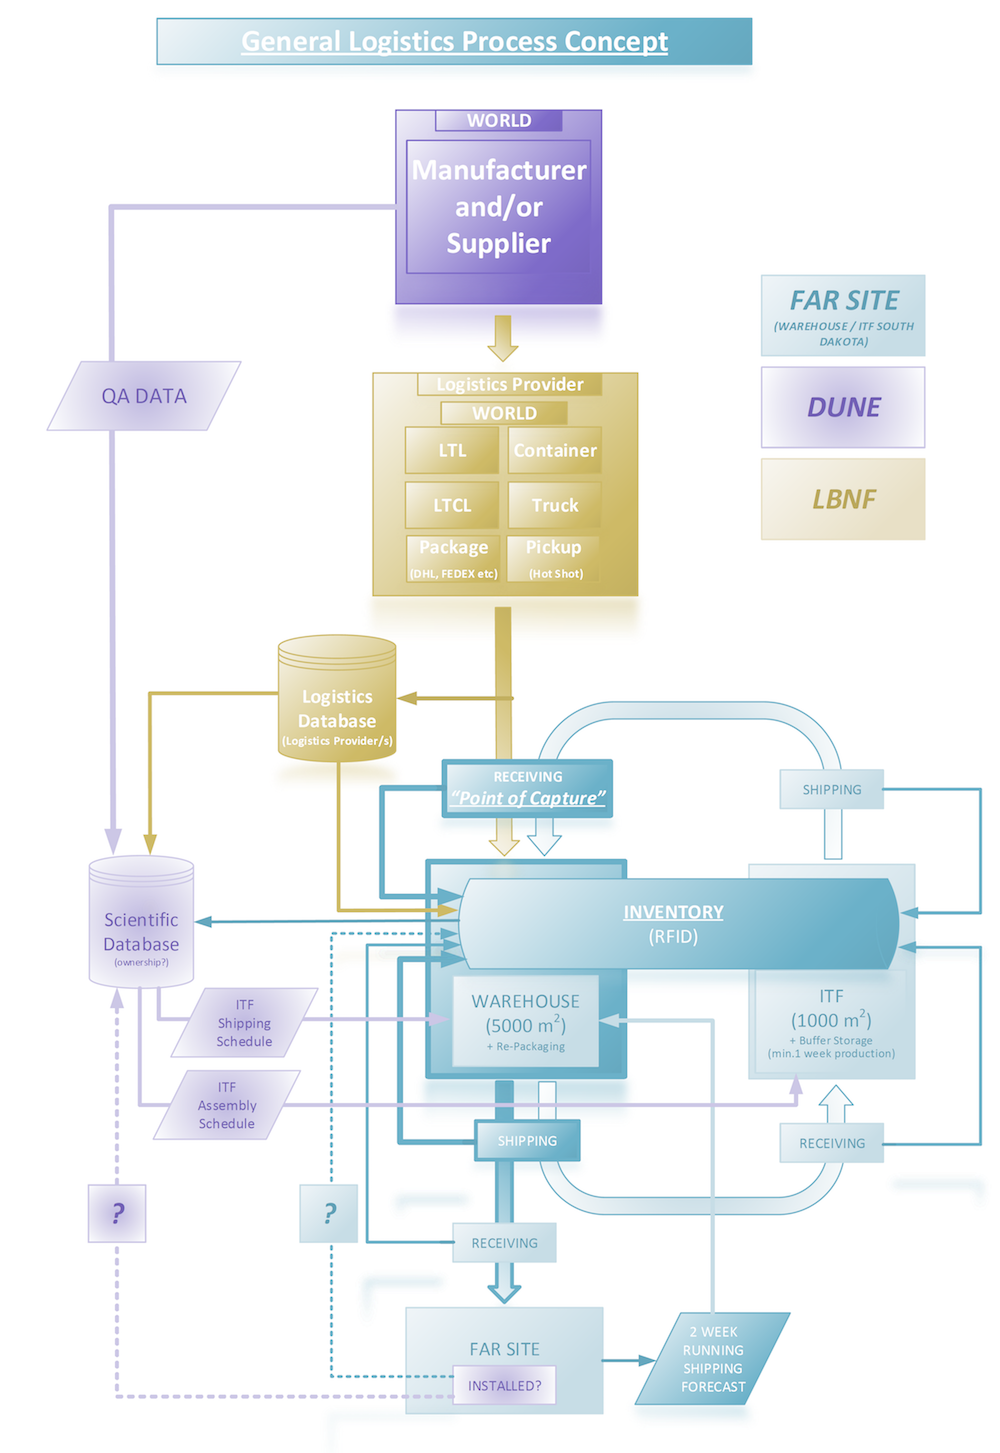
\includegraphics[width=0.85\textwidth]{logistics.png}
\end{dunefigure}
Within the cavern items provided by LBNF are represented on the left
and the items provided by DUNE are represented on the right. In
addition, \dword{tc} engineering team is also responsible for the
integration of the DAQ room in the Central Utility Cavern and surface
control and network room. Interfaces with LBNF are managed at the
boundaries of each integration node.

(Note: Write a short paragraph for each figure)


Figure~\ref{fig:detector_cavern} shows the detector within the cavern.
Caption: Overall view of the Detector within the cavern
\begin{dunefigure}[Overall view of the Detector within the cavern.]{fig:detector_cavern}
  {Overall view of the Detector within the cavern.}
%  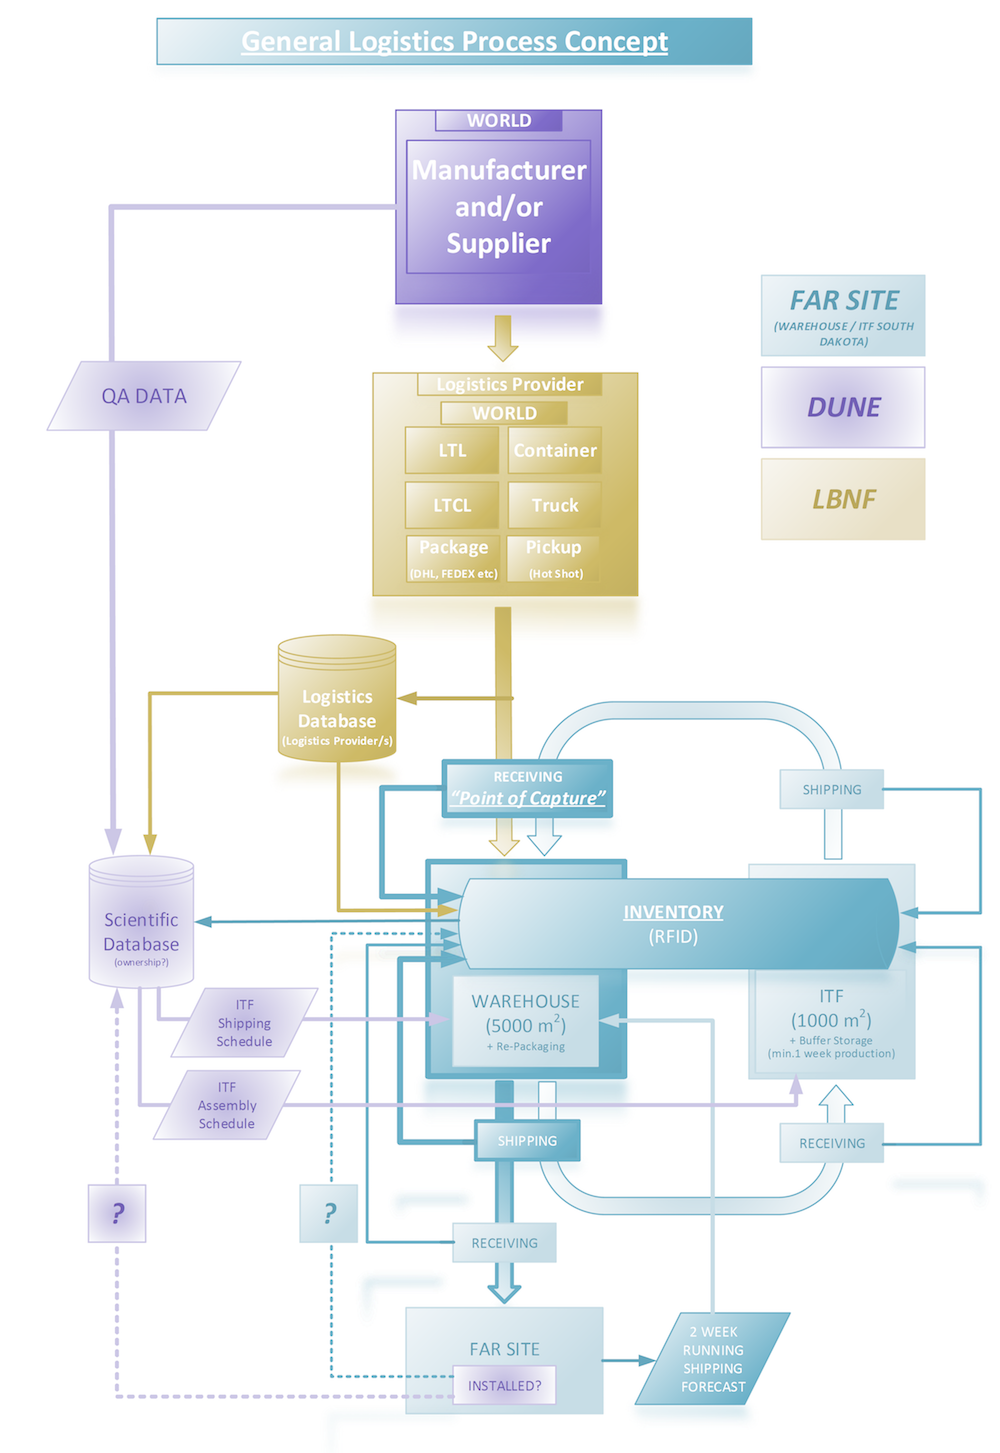
\includegraphics[width=0.85\textwidth]{logistics.png}
\end{dunefigure}

Figure~\ref{fig:detector_ew_elevation} shows the elevation view of the
detector within the cavern from east to west.  Caption: Overall view
of the Detector within the cavern
\begin{dunefigure}[East-west elevation view of Detector within the cavern.]{fig:detector_ew_elevation}
  {East-west elevation view of Detector within the cavern.}
  %  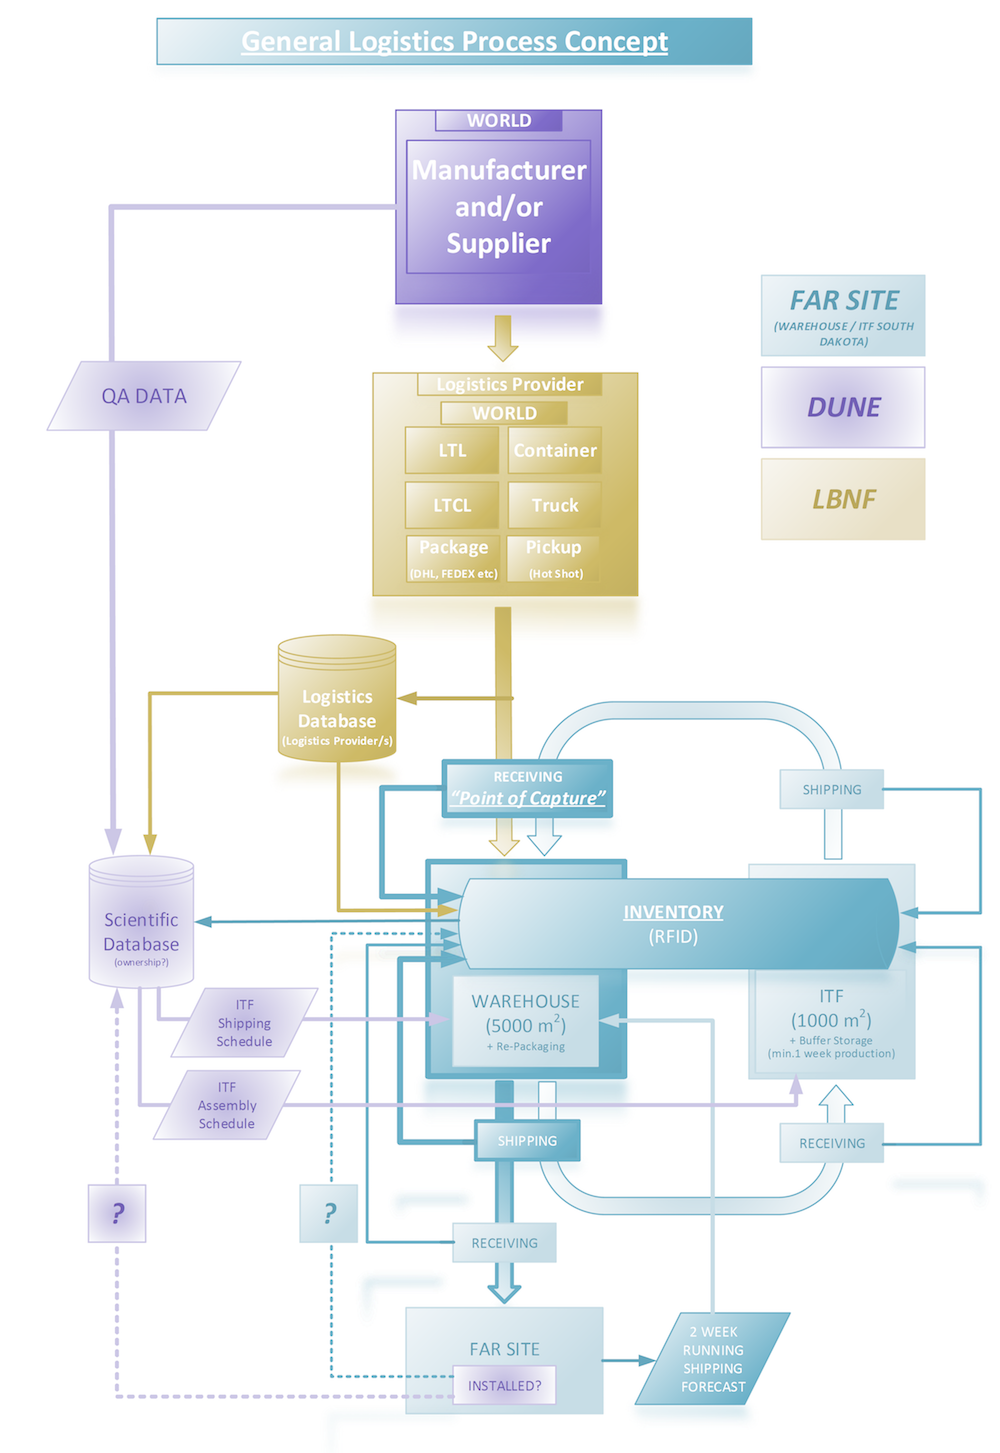
\includegraphics[width=0.85\textwidth]{logistics.png}
\end{dunefigure}

Figure~\ref{fig:detector_ns_elevation} shows the elevation view of the
detector within the cavern from north to south.
\begin{dunefigure}[North-south elevation view of Detector within the cavern.]{fig:detector_ns_elevation}
  {North-south elevation view of Detector within the cavern.}
  %  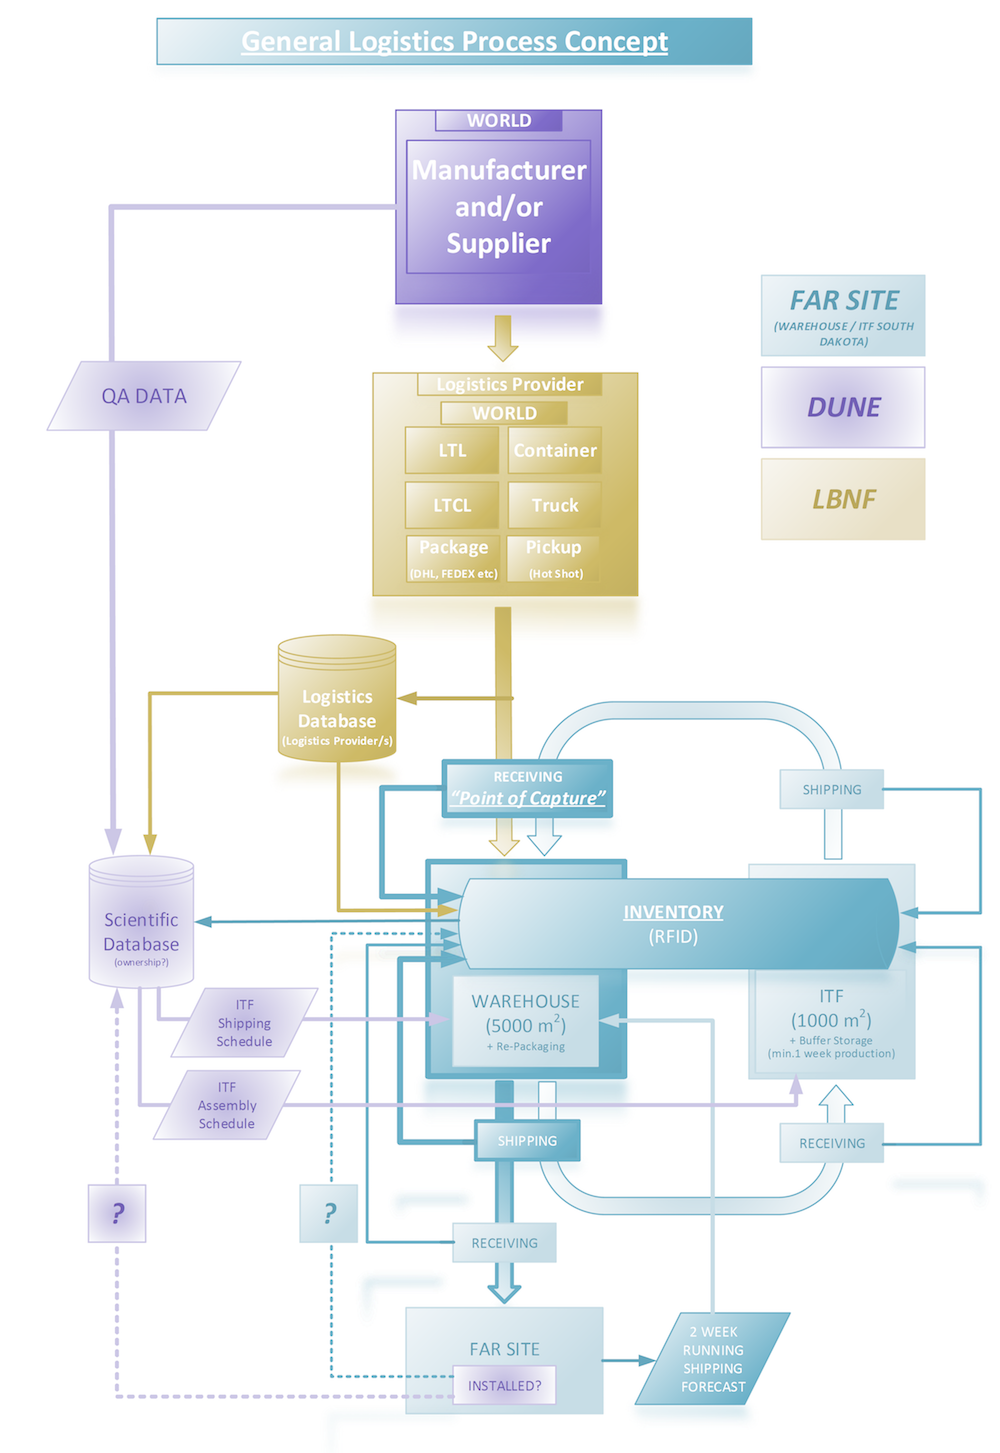
\includegraphics[width=0.85\textwidth]{logistics.png}
\end{dunefigure}



Figure~\ref{fig:detector_mezzanines} shows the elevation view of top
of cryostat showing mezzanines, cryogenic equipment and electronic
racks.
\begin{dunefigure}[Elevation view of top of cryostat showing mezzanines, cryogenic equipment and electronic racks.]{fig:detector_mezzanines}
  {Elevation view of top of cryostat showing mezzanines, cryogenic
    equipment and electronic racks.}
  %  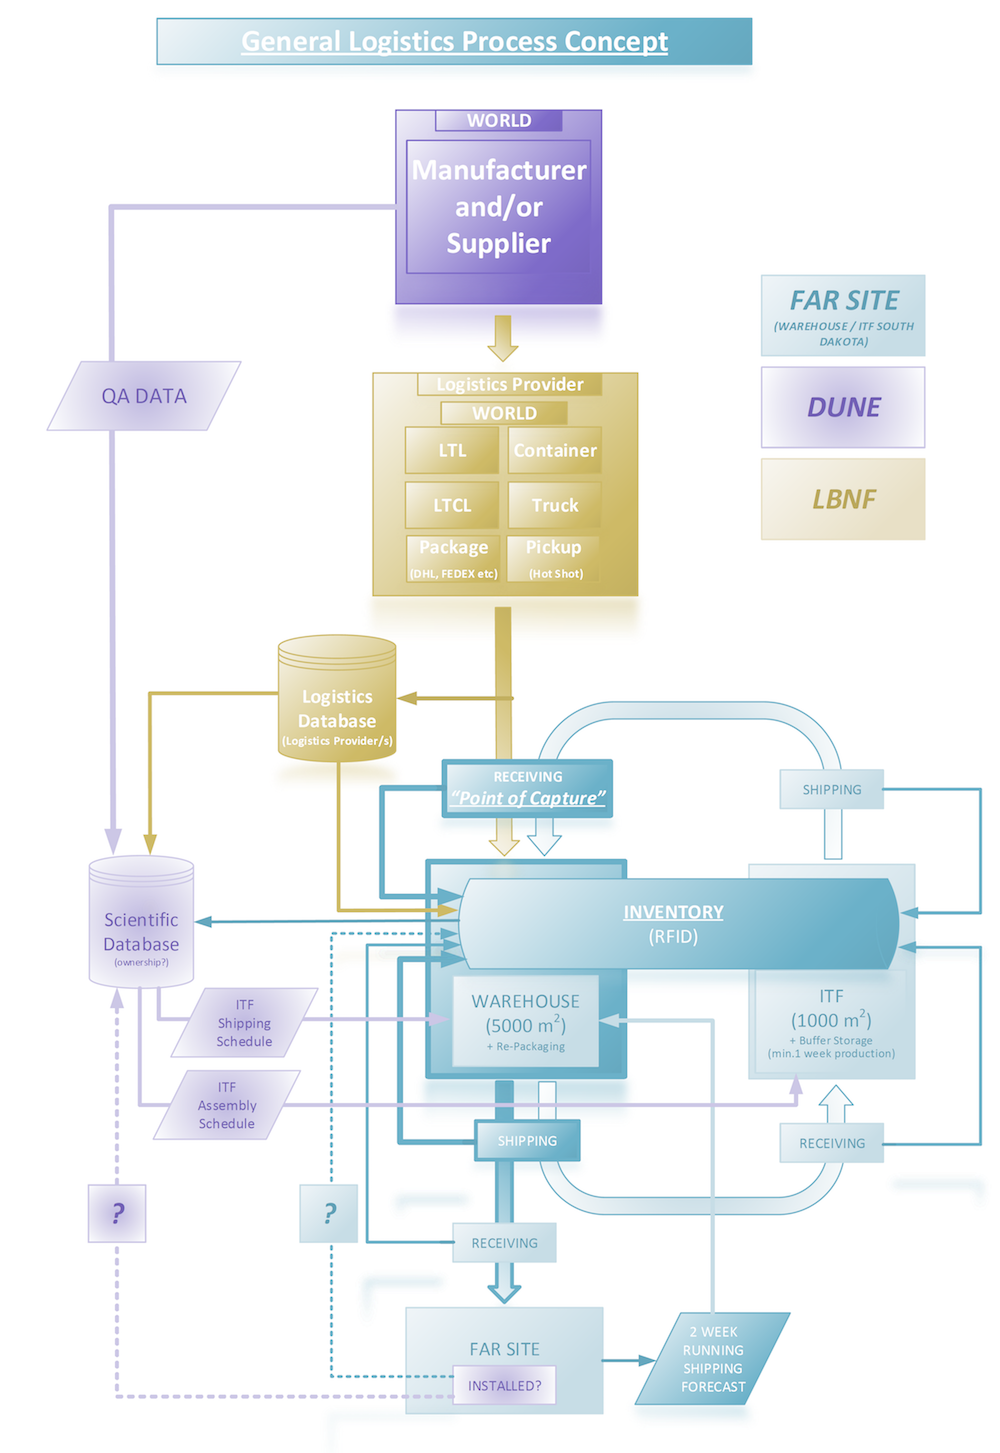
\includegraphics[width=0.85\textwidth]{logistics.png}
\end{dunefigure}

Figure~\ref{fig:detector_daq_floor_layout} shows the floor layout of underground DAQ room.
\begin{dunefigure}[Floor layout of underground DAQ room.]{fig:detector_daq_floor_layout}
  {Floor layout of underground DAQ room.}
  %  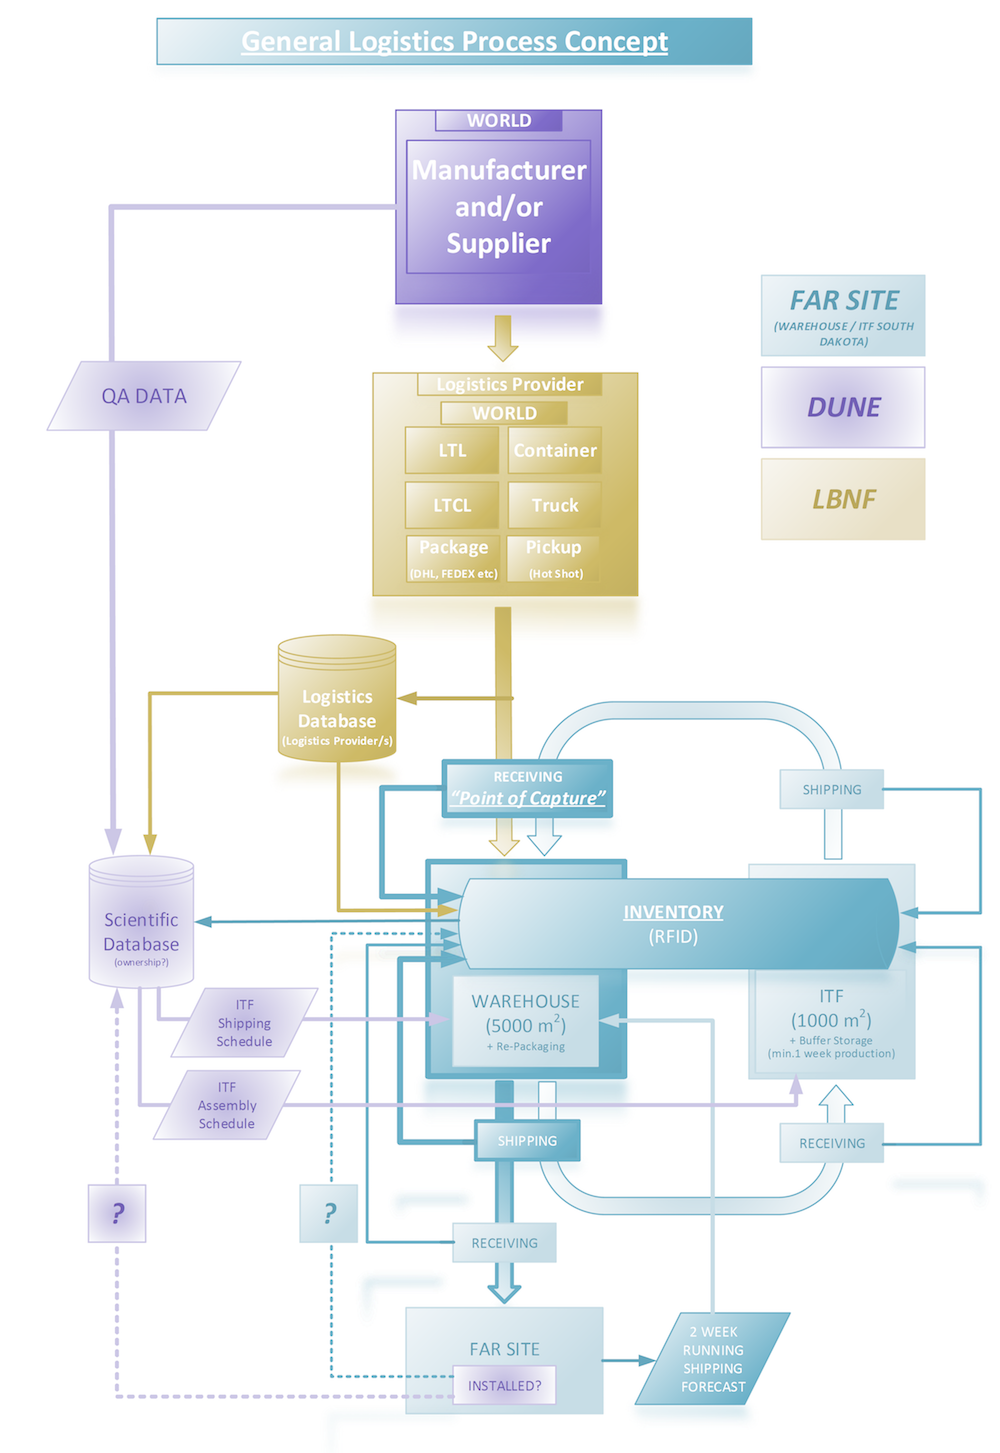
\includegraphics[width=0.85\textwidth]{logistics.png}
\end{dunefigure}

Figure~\ref{fig:detector_surface_floor_layout} shows the floor layout
of underground DAQ room.
\begin{dunefigure}[Floor layout of surface control and network room.]{fig:detector_surface_floor_layout} {Floor layout of surface control and network room.}
  % 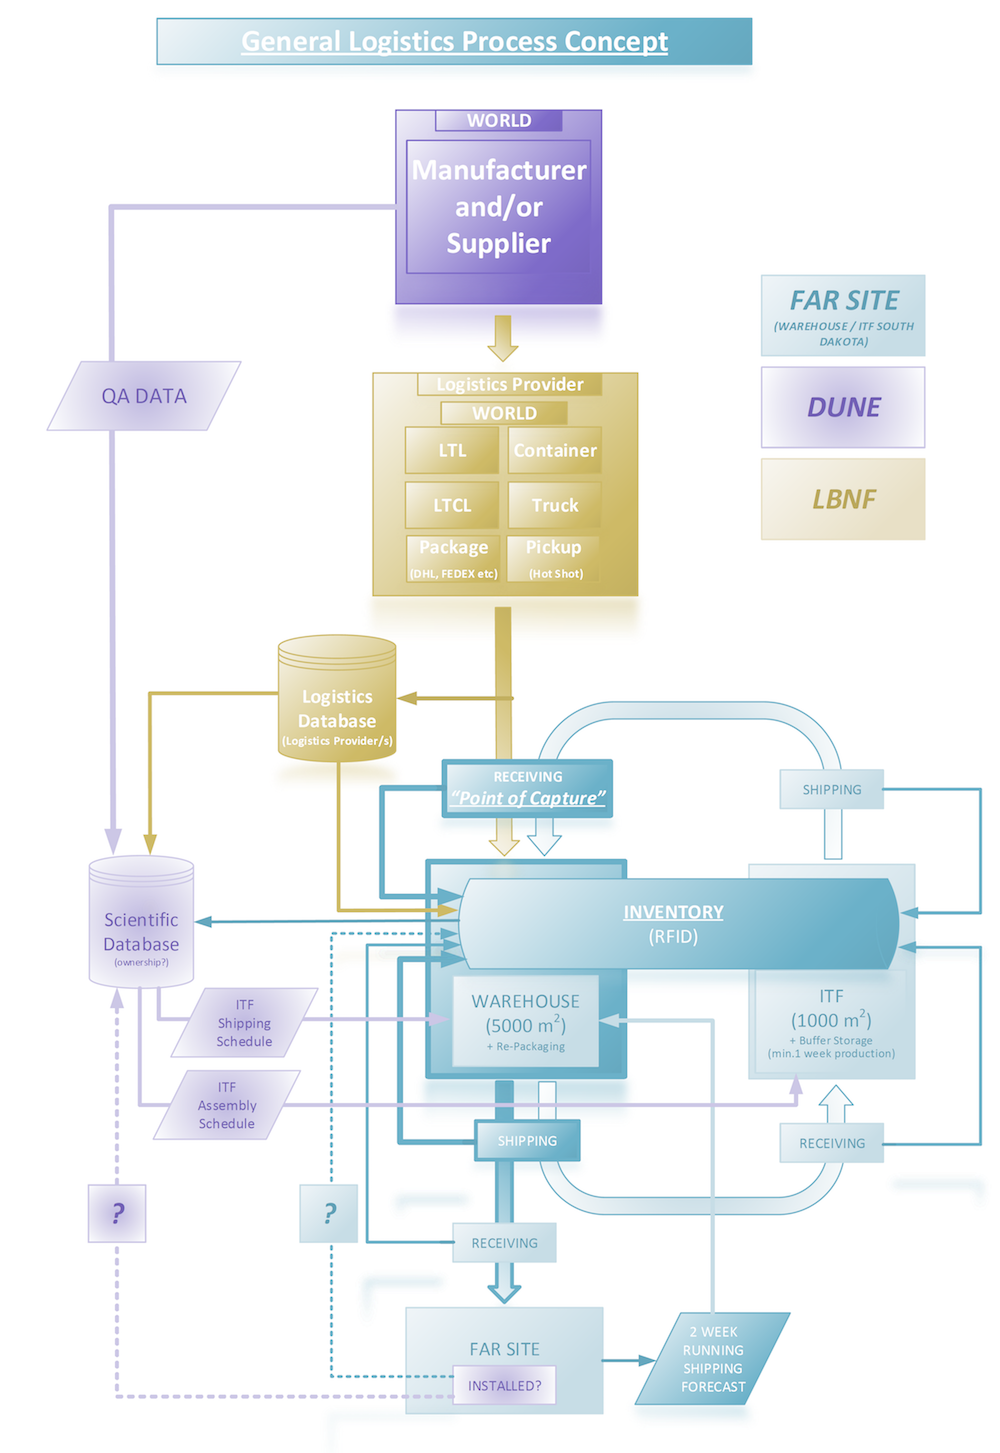
\includegraphics[width=0.85\textwidth]{logistics.png}
\end{dunefigure}

Figs:
Captions: Grounding, power interfaces, etc. 
Figure~\ref{fig:detector_grounding} shows grounding and power interfaces.
\begin{dunefigure}[Grounding and power interfaces.]{fig:detector_grounding} {Grounding and power interfaces.}
  % 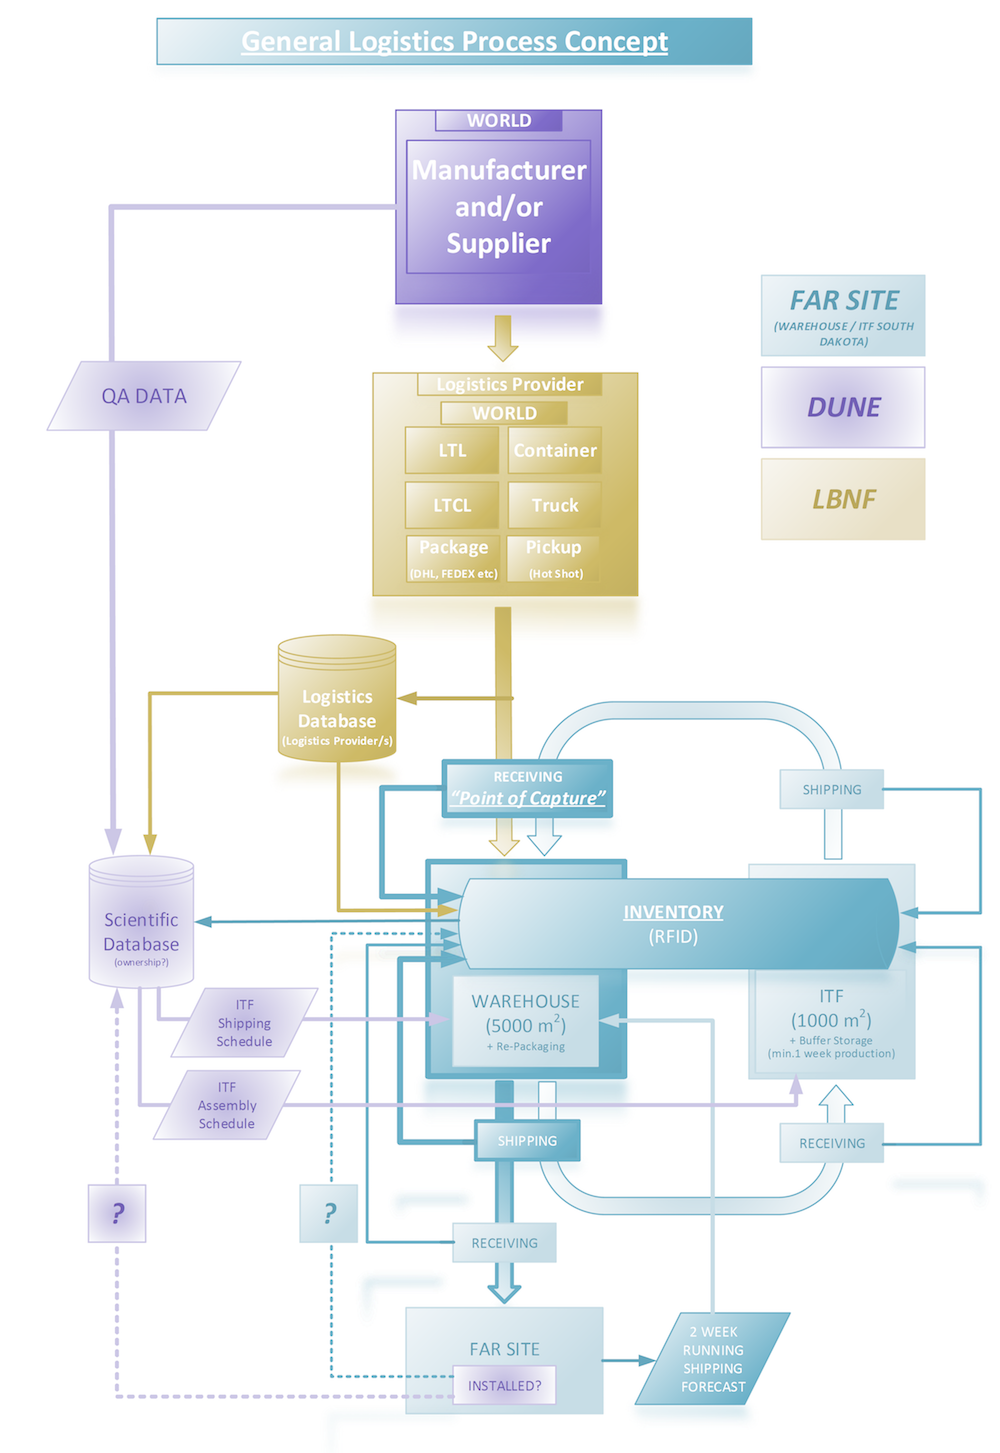
\includegraphics[width=0.85\textwidth]{logistics.png}
\end{dunefigure}

\section{Coordination}

...Method for determining and controlling interfaces with LBNF including conventional facilities

\section{Integration Drawings}

...This section shows all interfaces. Many will be needed with
dimensions and explanation. It will include all the interfaces between
detector and LBNF supplied items: e.g. DSS to CS, rack placement,
grounding, cable trays, cooling interfaces, power interfaces, DAQ
room, above ground control room and network etc...
